%%%%%%%%%%%%%%%%%%%%%%%%%%%%%%%%%%%%%%%%%%%%%%%%%%%%%%%%%%%%%%%%%%%%%
% LaTeX Template: Project Titlepage Modified (v 0.1) by rcx
%
% Original Source: http://www.howtotex.com
% Date: February 2014
% 
% This is a title page template which be used for articles & reports.
% 
% This is the modified version of the original Latex template from
% aforementioned website.
% 
%%%%%%%%%%%%%%%%%%%%%%%%%%%%%%%%%%%%%%%%%%%%%%%%%%%%%%%%%%%%%%%%%%%%%%

\documentclass[11pt]{article}
%\usepackage[a4paper]{geometry}
\usepackage[left=1.5cm,right=1.5cm,top=2cm,bottom=2cm]{geometry}

\usepackage[table,xcdraw]{xcolor}
\definecolor{ocre}{RGB}{243,102,25}
\usepackage{fancyhdr}
\usepackage{lastpage}
\usepackage{graphicx, wrapfig, setspace, booktabs}
\usepackage{titlepic}
\usepackage[T1]{fontenc}
\usepackage[font=small, labelfont=bf,center]{caption}
\usepackage{fourier}
\usepackage[protrusion=true, expansion=true]{microtype}
\usepackage[english]{babel}
\usepackage{sectsty}
\usepackage{url, lipsum}
\usepackage{multirow}
\usepackage{float}
\usepackage{amsmath}
\usepackage{bm}
\usepackage{subfig}
\usepackage{tikz}
\usepackage{svg}
\usepackage{filecontents}
\begin{filecontents*}{batch_rotode_des_flp2_pclab_quad.m}
   function dydx=fcn_ode(x,y,lambda)
      % FIELD EQUATION: rotating flapping blade
      z=y(1);                      % shape
      u=y(2);                      % diff shape
      v=y(3);                      % diff diff shape
      w=y(4);                      % diff diff diff shape
      EI=(168/L^2)*x^2-(336/L)*x+200;
      EId=(336/L^2)*x-(336/L);
      EIdd=(336/L^2);
      Tx=0.5*m*(L^2-x^2);
      Txd=m*x;
      % model for bvp4c
      dydx = [ ...
         u ; ...
         v ; ...
         w ; ...                   % Euler-Bernoulli flapping model
         (Omega^2*Tx*v+Omega^2*Txd*u+lambda*m*z-2*EId*w-EIdd*v)/(EI)];
         %(lambda*m*z+Omega^2*((0.5*m*(R^2-x^2)+mtT*R)*v-m*x*u))/EIf];
   end
\end{filecontents*}

\begin{filecontents*}{bc.m}
      % variable BC root
      if is_spring, cond1=va-(kf/200)*ua; % moment continuity
      else          cond1=ua;      % zero slope
\end{filecontents*}
\newcommand*{\lstconsolas}{\fontfamily{Consolas}\selectfont}
\usepackage[numbered,framed]{matlab-prettifier}
\usepackage[font={color=black},figurename=Fig.,labelfont={it}]{caption}
%\usepackage{titlesec}
%\titleformat{\section}
%  {\normalfont\fontsize{12}{15}\bfseries}{\thesection}{1em}{}
%\titlespacing*{\section}
%{0pt}{1}{1}
\usepackage{titling}

\setlength{\droptitle}{-7em}
\newcommand\ph\mlplaceholder

\renewcommand{\lstlistingname}{Matlab Code}% Listing -> Algorithm
\renewcommand{\lstlistlistingname}{List of \lstlistingname s}% List of Listings -> List of Algorithms
\newcommand{\HRule}[1]{\rule{\linewidth}{#1}}
\onehalfspacing
\setcounter{tocdepth}{5}
\setcounter{secnumdepth}{5}
\renewcommand{\baselinestretch}{1.5}
%-------------------------------------------------------------------------------
% HEADER & FOOTER
%-------------------------------------------------------------------------------
\pagestyle{fancy}
\fancyhf{}
\setlength\headheight{15pt}
\fancyhead[L]{iz16368}
\fancyhead[R]{University of Bristol}
\fancyfoot[R]{Page \thepage\ of \pageref{LastPage}}
%-------------------------------------------------------------------------------
% TITLE PAGE
%-------------------------------------------------------------------------------

\begin{document}
\title{ \normalsize \textsc{Dynamics of Rotors}
		\\ 		University of Bristol \\
		\HRule{1pt}
		\LARGE \textbf{\uppercase{Modal Analysis of Rotor Blade Structure}}
		\HRule{2pt} \normalsize}
		\vspace{-1cm}
\author{\vspace{-1cm}Ismaeel Zaman}
\maketitle

%-------------------------------------------------------------------------------
% Section title formatting
%\sectionfont{\scshape}
%-------------------------------------------------------------------------------

%-------------------------------------------------------------------------------
% BODY
%-------------------------------------------------------------------------------

\section*{Executive Summary}
%1/4 page brief description of activities, purpose, findings, conclusions
Rotor blade modal analysis is critical to ensuring that undesirable resonance does not occur.
This report investigates the experimental and computational aspects of this analysis. An impact modal analysis was carried out using a cantilevered beam and different root and tip conditions. It was found that as the root became less restrictive the damping increased, and as tip mass increased the modal frequencies reduced.The results were used to refine a MATLAB model of a hinged blade system. The model results differed from the experiment by up to $6.68\%$. The model was then used to produce a frequency diagram for a range of rotor speeds. Finally, to gain a deeper understanding of the workings of the $bv4c$ BVP solver the stiffness of the beam was described as varying across the span  through a constant, linear and quadratic distribution. The result of each of these were compared and it was found that as the order increased the resulting modal frequency and amplitude reduced. Future work may include additional testing of variable stiffness boundary conditions to determine true causes of observed trends. Also, a more controlled experiment to obtain more reliable data would be beneficial.
\section{Introduction}
%1/3 page  overall motivation, background, context, approach, procedures, aim and objectives
Dynamic modal analysis of rotor blades constitutes a very important aspect of blade design. It is vital in ensuring that the oscillation frequencies of each mode do not coincide with the natural rotor frequency as this would cause catastrophic failure. However determining the modal frequencies is no trivial matter and several different methods have been developed over the years. The problem is normally described by Ordinary Differential Equations and known conditions at boundaries. However, as opposed to an Initial Value Problem a Boundary Value Problem such as this is more complex to solve. Dynamic computational models that have been developed and validated through empirical data have been used to estimate these frequencies and overcome the BVP problem using functions such as $bvp4c$ which is the method employed in this report. Initially, an experiment was performed to investigate and gain understanding of the blade analysis and trends. This data would then be used to validate a computational model, adopting assumptions and idealisations. This model would then be modified to explore a more complex BVP problem in order to gain an understanding in the BVP method for such a structure.
\section{Experimental Phase}
%3-4 pages
\subsection{Experimental Setup}
%Purpose, specific research objectives, tasks, steps, procedures, …
The aim of this experiment is to obtain practical experience and understanding of experimental modelling and modal analysis of a rotor blade structure and to obtain data which could be later used to refine a computational model.\\
To achieve this aim the following objectives are set:
\begin{itemize}
\itemsep0em
    \item Determine natural frequencies in the selected frequency range for the range of configurations.
    \item Determine damping ratios for the first mode 
    \item Note the specifications of the test structure and conditions for later modelling.
    \item Discuss experiment and findings
\end{itemize}{}

\subsection{Experimental Modal Analysis}
%Blade structure, analysis method, inputs / outputs, test conditions and parameters, measured quantities, identified responses
The experiment modelled a stationary blade that was impacted and the structural deflection recorded for different root boundary conditions. This formed the basis of a rudimentary impact based modal analysis. \\
The displacement data was collected and analysed using Discrete Fourier Transform and the Logarithmic Decrement method to obtain the natural frequencies and damping ratios for the different conditions.\\
The apparatus consisted of an Aluminium beam with a hollow rectangular cross-section with dimensions in Figure \ref{fig:dim}, clamped to a rigid structure through a steel link.\\

\begin{figure}[H]
    \centering
    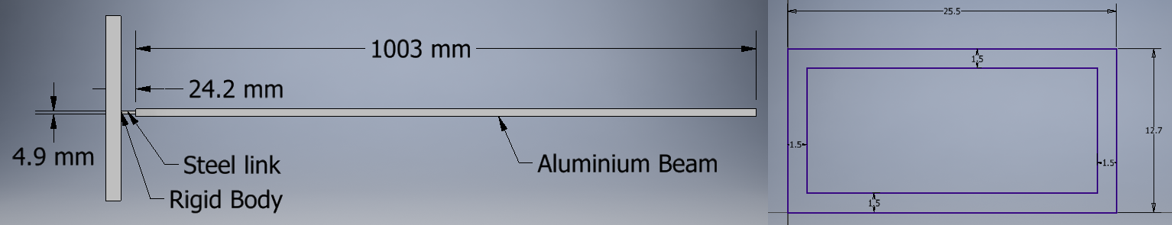
\includegraphics[width=0.9\textwidth]{dimensions.PNG}
    \caption{Dimensions of test structure}
    \label{fig:dim}
\end{figure}{}
For data measurement and acquisition a single channel \textit{Bruel\&Kjaer} piezoelectric accelerometer was fixed to the tip of the beam and was connected to a National Instruments NI 9234 signal analyser. This was linked to a Matlab program for data interpretation and storage. Figure \ref{fig:photo} shows an image of the setup.
\begin{figure}[H]
    \centering
    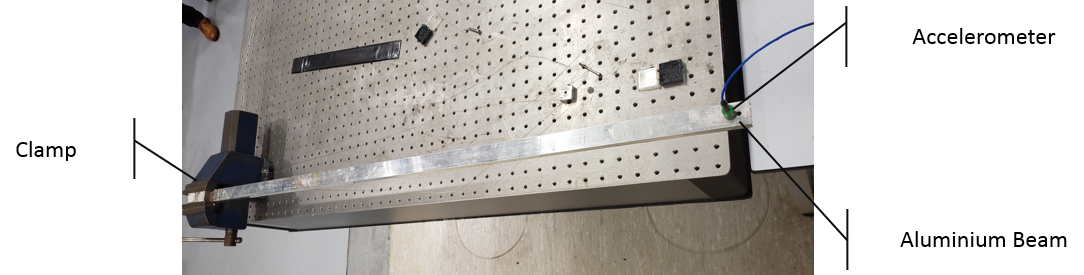
\includegraphics[width=0.9\textwidth]{photoedit.PNG}
    \caption{Photo showing experiment setup including aluminium beam in its 90 deg rotated position, accelerometer and clamp}
    \label{fig:photo}
\end{figure}{}

Initially, the beam was oriented so that the beam would deflect in a plane that was opposed by the clamp geometrically. The beam was deflected and released and the data recorded. The beam was then rotated 90 degrees about its span-wise axis and clamped tightly so that the restoring force produced comes from the friction between the clamp and the beam. The beam was deflected again and data recorded. The clamp was then loosened slightly and the experiment repeated.The next stage involved adding tip masses to the beam.
The orientation of the beam was reverted to its original state and aluminium and steel tip masses of 10g and 30g respectively, were added separately as well as a case of no tip mass. The masses were attached using Blu-Tack to the tip of the beam. The beam was impacted with a hard tipped hammer and the responses were recorded for each case.
Each case was repeated twice to reduce random error. Traditionally, this method of impact testing is performed in a controlled environment with force-measuring hammers to increase the accuracy and reliability of the data, this was not available here.
From the Discrete Fourier Transform plot, the modal frequencies were determined by selecting the data points at the obvious peaks. This method of impact testing is only accurate at relatively low frequencies due to the finite impulse duration which leads to the resulting excitation frequencies being limited, \cite{brano1}, so only the first three modes were taken.
To obtain the damping ratio, the time history plots were analysed, the outputs were very at an extremely high resolution and contained many nested oscillations, which meant that the $findpeaks$ function had to to have the Minimum Peak Distance set at a value of 0.08. The logarithmic decrement formula, $\zeta_{\text {exp }} \approx \frac{1}{2 \pi N} \ln \left(\frac{x\left(t_{1}\right)}{x\left(t_{1}+N T_{D}\right)}\right) \label{eq:logdec}$, was used to find the damping ratio.

However, it should be noted that the data behaves erratically and will produce different results depending on input parameters of the analysis, the values and precision of the values in question are extremely fine and the reliability and validity of the experiment setup may not have been sufficient to allow a high degree of confidence. It was observed that the damping values could vary by up to $20\%$.

\subsection{Results}
%Parameter, condition, result tables; graphs of measured changes, trends, differences; absolute / relative

The results for the modal frequencies and damping ratios for all cases can be seen in Table \ref{tab:1res}. The damping ratios for the tip mass cases are not expected to vary but are shown here for completeness.
\begin{table}[H]
\footnotesize
\caption{Table showing characteristics for all cases. "Geo" denotes the original beam orientation, "Friction" denotes the rotated orientation.}
\centering
\begin{tabular}{|c|c|c|c|c|}
\hline
\rowcolor[HTML]{CBCEFB} 
\cellcolor[HTML]{CBCEFB}                       & \cellcolor[HTML]{CBCEFB}                                         & \multicolumn{3}{c|}{\cellcolor[HTML]{CBCEFB}Modal Frequencies (Hz)} \\ \cline{3-5} 
\rowcolor[HTML]{CBCEFB} 
\multirow{-2}{*}{\cellcolor[HTML]{CBCEFB}Case} & \multirow{-2}{*}{\cellcolor[HTML]{CBCEFB}Damping Ratio, $\zeta$} & F1                   & F2                   & F3                    \\ \hline
Free Geo Clamped                               & 0.001566                                                         & 11.10                & 72.06                & 206.13                \\ \hline
Free Friction Tight                            & 0.002904                                                        & 11.14                & 71.83                & 205.95                \\ \hline
Free Friction Loose                            & 0.003900                                           & 11.11                & 71.58                & 204.60                \\ \hline
Impact Geo No Tip Mass                         & 0.001365
                                                       & 11.16                & 72.09                & 206.42                \\ \hline
Impact Geo 10g Tip Mass                        & 0.001341                                                         & 10.60                & 69.22                & 200.17                \\ \hline
Impact Geo 30g Tip Mass                        & 0.001464                                                         & 9.71                 & 65.58                & 193.21                \\ \hline
\end{tabular}
\label{tab:1res}
\end{table}
% \begin{figure}[H]
%     \centering
%     \subfloat[Full response showing damped oscillation]{{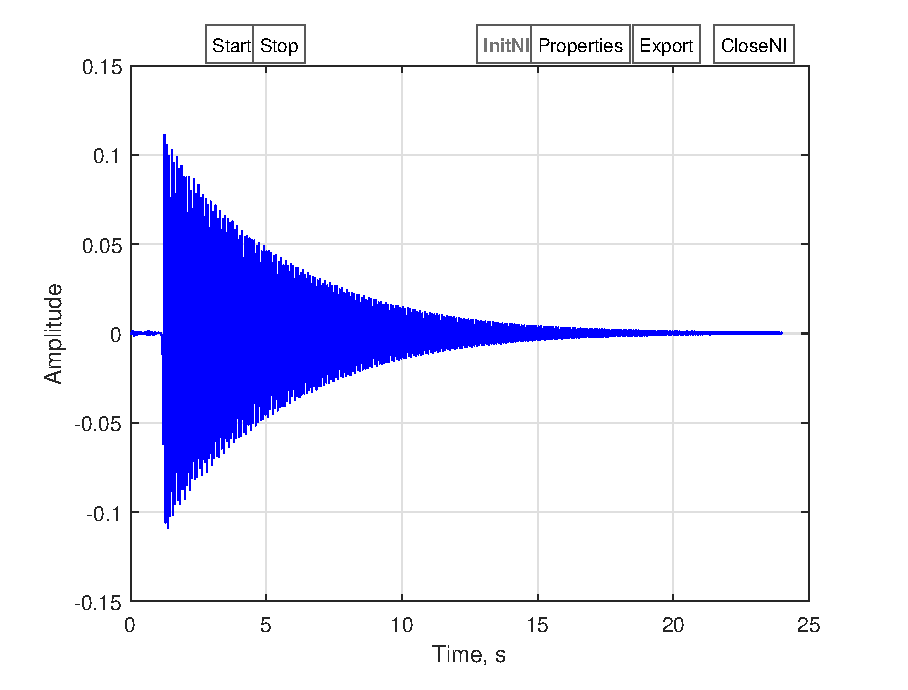
\includegraphics[width=0.44\textwidth]{TS1.eps}}}
%     \qquad
%     \subfloat[Enlarged section]{{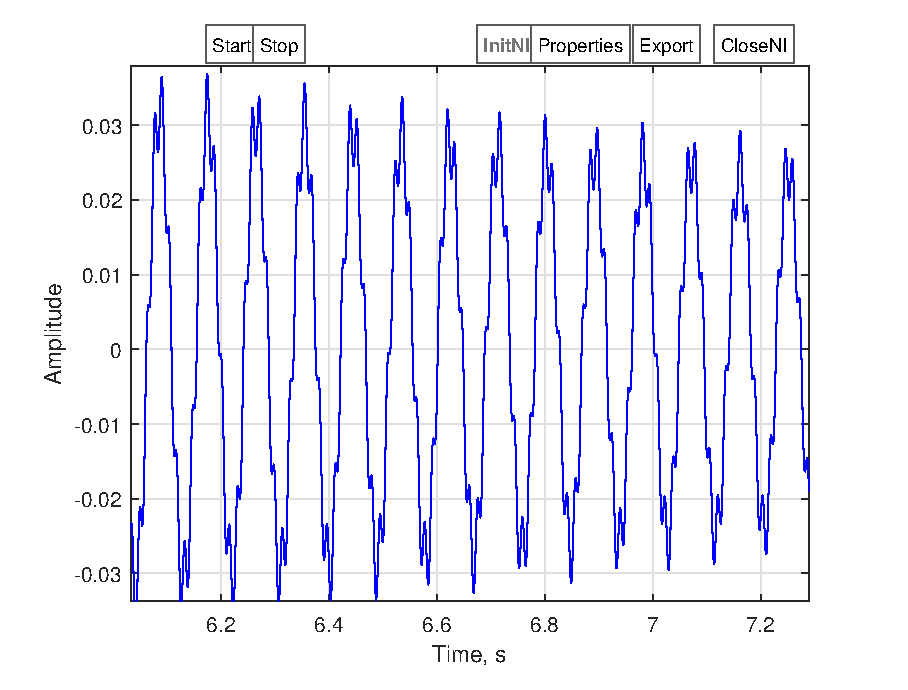
\includegraphics[width=0.44\textwidth]{TS2.eps}}}
%     \caption{Time history plot of the "free friction tight" response}
%     \label{fig:TS}
% \end{figure}
\subsection{Discussion}
%Experimental discussion, insights based on trends and effects, physical reasons, further use, …

From Table \ref{tab:1res}, it can be seen that the effect of rotating the beam so that the oscillation is opposed by friction is that the damping ratio increases, this could be due to the micro-displacements at the root dissipating energy quicker. The damping ratio increases again when the clamp is loosened slightly, this could be due to the same reasons of larger root displacements causing larger energy dissipation and quicker damping. It is observed that the modal frequencies do not vary significantly during these changes and can be said to remain constant or reduce slightly.
As the mass at the tip is increased, the natural frequencies of the modes reduce. This agrees with the theory, that as mass is added the natural frequencies reduce. It was also observed that the damping ratios did not vary significantly, as expected. The experiment relied on obtaining very sensitive and fine readings which would normally require a fully isolated system, however, in this case the experiment was performed in a busy environment where footsteps, other experiments, breathing could affect and interfere with the results. It should also be noted that the method for inducing vibration was done by hand and could not be confirmed to be consistent between tests. This could also be a contributing factor in introducing error.

\section{Blade Modelling}
%3-4 pages 
\subsection{Blade Model}
%Purpose (with ref. to section 1), specific research objectives, tasks, steps, procedures …
From the results in Part 1 it was possible to refine a computational MATLAB model of a rotor blade structure to as close as possible match the response of the experiment.
The aim of this section is to develop an understanding of the computational aspect of modal analysis with respect to a rotor blade structure.

The objectives to be achieved are :

\begin{itemize}
\itemsep0em
    \item Use experimental results and specifications to refine and validate a MATLAB model.
    \item Generate frequency diagrams for a range of flapping modes and rotor speeds
    \item Analyse results and discuss findings
\end{itemize}{}

\subsection{Computational Modal Analysis}
%Blade model, assumptions, analysis method, conditions and parameters, solver, computed responses
The model assumes a cantilevered beam with a specified hinge offset. The stiffness and dimensions of the rotor (beam) are input parameters as well as the root stiffness, an equivalent torsional spring. The model can account for tip masses and output mode-shapes and modal frequencies.\\
The model uses the MATLAB function \textit{bvp4c} which is discussed further in the next section.
However, the main difficulty in modelling a cantilever beam as a hinged blade comes from the assumptions and boundary conditions used. The model assumes a beam with a specified hinge offset and a rotational stiffness at that hinge. This stiffness constitutes the main root boundary condition and care must be taken when estimating this value. The effective hinge offset plays a large role in the resulting physics of the problem and for a cantilever beam, methods such as using Southwell's coefficient from charts in \cite{charts} to estimate this value could be used. However, for this experiment there exists a natural "hinge" location as there is a large discontinuity in stiffness near the root contributed by the steel link. Therefore, this measured location of the transition between steel and aluminium was used as the position of the hinge. Leaving the root stiffness to be the variable that could be refined. Another boundary condition is the mass at the tip, the experiment investigated cases where there was no tip mass, a 10g tip mass and a 30g tip mass. The model takes this into account and also smoothens the shear discontinuity introduced by a tip mass.

The dimensions of the physical experimental setup can be seen in Figure \ref{fig:dim}, with the beam dimensions, $1003 \times 25.5 \times 12.7 mm$ and a wall thickness of $1.5 mm$. From this, and an estimate of $E=70GPa$ for Aluminium, it was possible to calculate the flapping stiffness of the beam $EI$. However, an additional parameter is required in the form of the root stiffness. This value was initially based on the stiffness of the steel link. The relationship was derived from equations from beam theory:
\begin{align}
    \theta=\frac{Ml}{EI},& \text{ and }
    k=\frac{M}{\theta}\\
    \text{therefore}, k&=\frac{E_s I_s}{l_s}
\end{align}{}
where $M$ is the moment applied, $l$ is the length of the beam, $E$ is the Young's Modulus, $I$ is the second moment of area of the cross-section and $K$ is the beam stiffness. The steel link had dimensions of $24.5 \times 22.2 \times 4.9 mm$, A Young's Modulus for steel was estimated to be $210GPa$ and thus the $E_s I_s$ was calculated, giving $k=1.866e+03$. This value was used as a starting point was iterated to empirically obtain results that more closely match the experimental results. Using a value of $60\%$ of the initial $k$ produced results that had large agreement as can be seen in Table \ref{tab:lab2res}. A plot was generated that shows the flapping frequencies of the first six modes as they vary with rotor speed, from $0$ to $1800 rpm$. This can be seen in Figure \ref{fig:freqdiag}. Additionally, the relative frequency margin between each harmonic mode  and the rotor natural frequency was plotted at a rotor rpm of $568$, which is close to a standard rotor speed. This plot can be seen in Figure \ref{fig:reldiff}. Curve fitting was attempted to determine the trend.

\subsection{Results}
%Computed versus measured frequencies; absolute / relative frequency differences, trends; graphs and tables; frequency diagram and measured data, rotor harmonics, frequency separation …
\begin{figure}[H]
    \centering
    \subfloat[\label{fig:freqdiag} Diagram showing how the first six modal frequencies vary with rotor speed]{{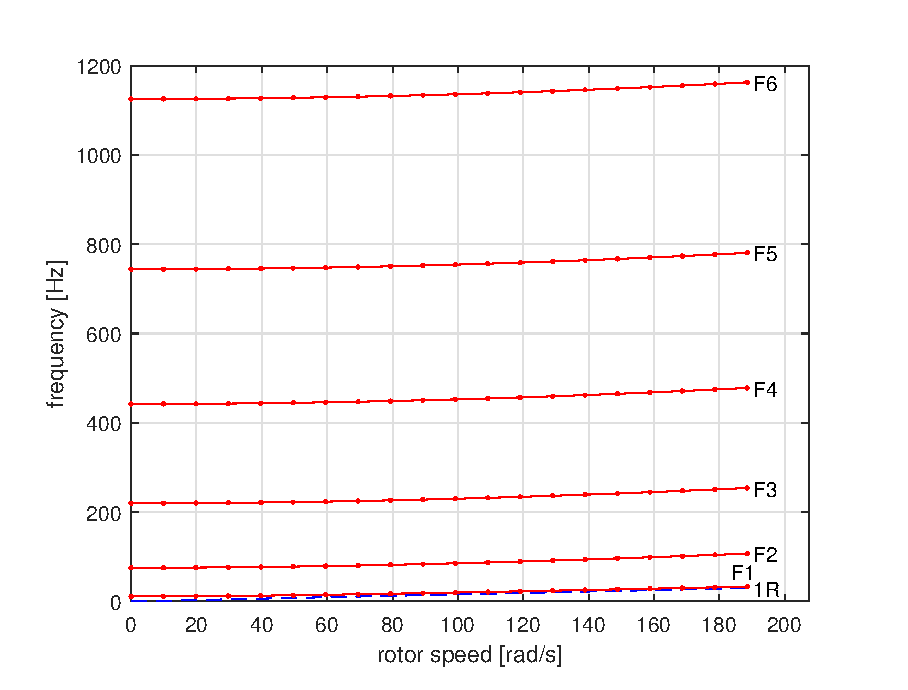
\includegraphics[width=0.45\textwidth]{FREQDIAG.eps}}}
    \qquad
    \subfloat[\label{fig:reldiff}Plot of the frequency margins for each harmonic, from the natural rotor frequency, with fitted curve]{{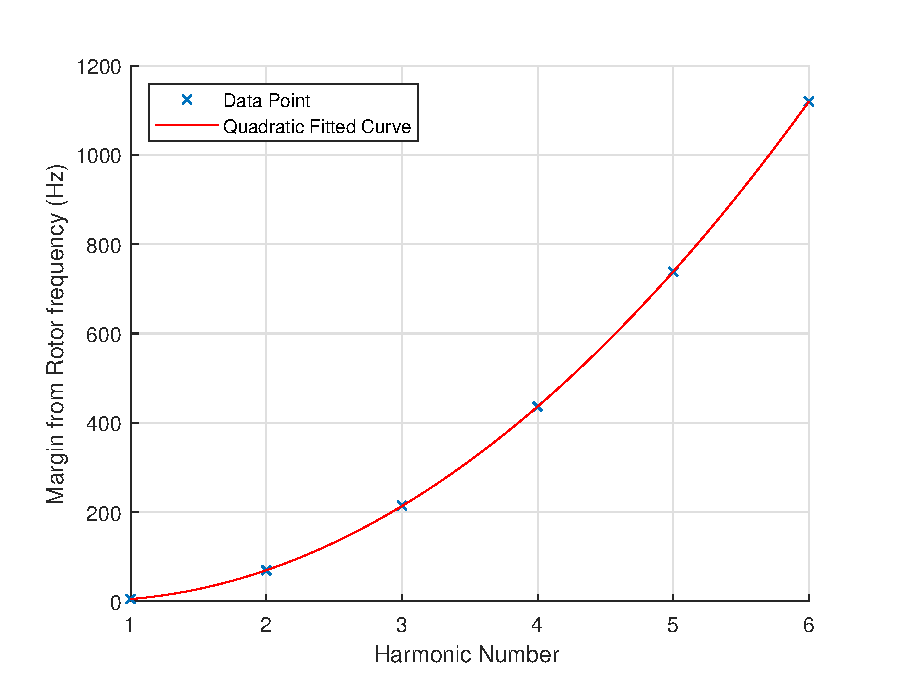
\includegraphics[width=0.45\textwidth]{RelDiff.eps}}}
    \caption{Frequency diagram and relative difference plots of the first six harmonics (no tip mass)}
\end{figure}

\begin{table}[H]
\scriptsize
\centering
\caption{Table showing modal frequencies results of computational model and comparison with experimental values.}
\begin{tabular}{|c|c|c|c|c|c|}
\hline
\rowcolor[HTML]{CBCEFB} 
\cellcolor[HTML]{CBCEFB}                       & \cellcolor[HTML]{CBCEFB}                                                                                                 & \multicolumn{2}{c|}{\cellcolor[HTML]{CBCEFB}Inital $k$ estimate}                                                                              & \multicolumn{2}{c|}{\cellcolor[HTML]{CBCEFB}Refined $k$ estimate}                                                                                \\ \cline{3-6} 
\rowcolor[HTML]{CBCEFB} 
\multirow{-2}{*}{\cellcolor[HTML]{CBCEFB}Case} & \multirow{-2}{*}{\cellcolor[HTML]{CBCEFB}\begin{tabular}[c]{@{}c@{}}Experimental \\ Modal Frequency\\ (Hz)\end{tabular}} & \begin{tabular}[c]{@{}c@{}}Model Modal \\ Frequency (Hz)\end{tabular} & \begin{tabular}[c]{@{}c@{}}Percentage \\ Difference (\%)\end{tabular} & \begin{tabular}[c]{@{}c@{}}Model Modal\\  Frequency\\  (Hz)\end{tabular} & \begin{tabular}[c]{@{}c@{}}Percentage\\  Difference (\%)\end{tabular} \\ \hline
\rowcolor[HTML]{C0C0C0} 
No Tip Mass                                    &                                                                                                                          &                                                                       &                                                                       &                                                                          &                                                                       \\ \hline
F1                                             & 11.1                                                                                                                     & 12.14                                                                 & \cellcolor[HTML]{FFFC9E}9.37                                                                  & 11.15                                                                    & \cellcolor[HTML]{FFFC9E}0.45                                                                  \\ \hline
F2                                             & 72.06                                                                                                                    & 78.9                                                                  & \cellcolor[HTML]{FFFC9E}9.49                                                                  & 75.49                                                                    &\cellcolor[HTML]{FFFC9E} 4.76                                                                  \\ \hline
F3                                             & 206.13                                                                                                                   & 225.96                                                                & \cellcolor[HTML]{FFFC9E}9.62                                                                  & 219.9                                                                    & \cellcolor[HTML]{FFFC9E}6.68                                                                  \\ \hline
\rowcolor[HTML]{C0C0C0} 
10.0g Tip Mass                    &                                                                                                                          &                                                                       &                                                                       &                                                                          &                                                                       \\ \hline
F1                                             & 10.59                                                                                                                    & 11.37                                                                 & \cellcolor[HTML]{FFFC9E}7.37                                                                  & 10.47                                                                    & \cellcolor[HTML]{FFFC9E}-1.13                                                                 \\ \hline
F2                                             & 69.23                                                                                                                    & 74.34                                                                 & \cellcolor[HTML]{FFFC9E}7.38                                                                  & 71.09                                                                    &\cellcolor[HTML]{FFFC9E} 2.69                                                                  \\ \hline
F3                                             & 200.17                                                                                                                   & 213.8                                                                 & \cellcolor[HTML]{FFFC9E}6.81                                                                  & 208.01                                                                   & \cellcolor[HTML]{FFFC9E}3.92                                                                  \\ \hline
\rowcolor[HTML]{C0C0C0} 
30.0g Tip Mass                         &                                                                                                                          &                                                                       &                                                                       &                                                                          &                                                                       \\ \hline
F1                                             & 9.7                                                                                                                      & 10.19                                                                 & \cellcolor[HTML]{FFFC9E}5.05                                                                  & 9.4085                                                                   &\cellcolor[HTML]{FFFC9E} -3.01                                                                 \\ \hline
F2                                             & 65.58                                                                                                                    & 68.9                                                                  & \cellcolor[HTML]{FFFC9E}5.06                                                                  & 65.847                                                                   &\cellcolor[HTML]{FFFC9E} 0.41                                                                  \\ \hline
F3                                             & 193.21                                                                                                                   & 202.19                                                                & \cellcolor[HTML]{FFFC9E}4.65                                                                  & 196.59                                                                   &\cellcolor[HTML]{FFFC9E} 1.75                                                                  \\ \hline
\end{tabular}
\label{tab:lab2res}
\end{table}


\subsection{Discussion}
%Model-experiment errors, modelling insights based on error trends, frequency diagram discussion …
From the results in Table \ref{tab:lab2res}, it can be seen that the initial estimate for root stiffness $k$ produced results that differed from experimental results by a maximum of $9.62\%$. It was observed that this initial value over estimated the natural frequencies so to provide lower results the $k$ value was decreased. The refined $k$ results differed from the experimental values by a maximum of $6.68\%$. It was observed that the error in the results increased as the mode number increased, suggesting that the mode was less accurate at higher frequencies. This trend was not observed for the $30.0g$ tip mass case however, the error increased, but the absolute value of the error did not. With the model largely underestimating the first harmonic. An additional trend was also observed, that the error of each respective harmonic increased negatively as the tip mass increased. This could be attributed the the hinge offset not being a true equivalent to the experiment setup or the fact that the Young's Modulus of the materials were estimated rather than determined.
From Figure \ref{fig:freqdiag}, it can be seen that as the rotor speed increases so do the modal frequencies. It is important that the modal frequencies do not intersect the natural frequency of the rotor otherwise resonance may occur and contributed to rapid unplanned disassembly of the rotor system. While the modal frequencies do not intersect the natural rotor frequency the first mode does come within $3Hz$, which is not ideal. The frequency margin of the modes from the rotor frequency was plotted in Figure \ref{fig:reldiff} and it was found the the trend fit a quadratic curve perfectly. To increase the margin the modal frequencies should be raised higher this could be done by increasing the root stiffness or decreasing the mass of the blade. Other methods could be to reduce the modal frequencies such that they never cross the 1R line upwards in the first place. However, for this case that would require large modifications.


\section{BVP Programming}
%2pages
\subsection{Programming Option: A}
%Purpose (with ref. to section 2), specific research objectives, tasks, steps, procedures …
The MATLAB model has been improved and validated in the previous section. This section will now investigate the Boundary Value Problem method, specifically with regards to the $bvp4c$ solver that is used in the model.\\
The aim of this part is to demonstrate the theoretical and computational sides of the BVP method for elastic blades. The objectives for this part are:

\begin{itemize}
\itemsep0em
    \item Implement the variable stiffness blade problem in MATLAB using the $bvp4c$ format.
    \item Analyse and compare the result of different stiffness distribution orders.
    \item Discuss findings
\end{itemize}

\subsection{Model Description}
%Matlab BVP format; field equations, boundary conditions, assumptions, analysis method, …
$bvp4c$ is a MATLAB BVP solver based on the collocation method, which is a version of Method of Weighted Residuals, \cite{bvp}. It finds unique solutions to ODEs with boundary values rather than initial values. It does this using the ODE field equation, the boundary conditions, a normalising factor to identify unique solutions and an initial guess.\\
The task required a change in the field equation to take into account a varying $EI$ along the span. The conditions were a hinged blade with a non-zero hinge offset, a free tip and a constant mass distribution.
The field equations need to be written as a set of $1^{st}$ Order ODEs, where terms of a higher order are substituted for an independent variable which is defined earlier in the code.
The solver requires the field equation to be defined by $w^{iv}$ and so for a variable $EI$ the result is Equation \ref{eq:field}. The code implementation can be seen in \textit{Matlab Code 1}.

\begin{equation}
    w^{iv}=\frac{\lambda \,m\,w-2\,\mathrm{EI^{'}}\,w^{'''}-\mathrm{EI^{''}}\,w^{''}+\Omega ^2\,\mathrm{Tx^{'}}\,w^{'}+\Omega ^2\,\mathrm{Tx}\,w^{''}}{\mathrm{EI}} \label{eq:field}
\end{equation}{}
\vspace{-1cm}
\lstinputlisting[style=Matlab-editor,basicstyle=\lstconsolas\small,caption=Implementation of Field Equation,linerange={13-17}]{batch_rotode_des_flp2_pclab_quad.m}

The stiffness distribution was modelled as a constant distribution, a linear distribution and a quadratic distribution. To decide the coefficients of the equation that describes each it was assumed there existed a physical beam with a known non-linear stiffness distribution. The stiffness values at $x=0$ and $x=l$ are known as well as the gradient at the latter.
If a \textit{constant} stiffness distribution was desired the value would be idealised as the average of the two values. If a \textit{linear} stiffness distribution was desired it would be idealised at a straight line joining the values at the ends of the beam. If a \textit{quadratic} stiffness distribution was desired then the addition of a zero gradient at $x=l$ would be introduced.\\
A blade with root $EI_r=200Nm$ and a taper ratio of $0.737$ gives a tip $EI_t=32$, it is assumed that $\frac{dEI}{dx}=0\,|\,x=l$ and $l=1.003\,m$
Therefore, the $EI(x)$ equations for each distribution are:
\begin{align}
    Constant: \,\,EI(x)&=116\\
  Linear:\,\,  EI(x)&=200-\frac{168x}{l}\\
  Quadratic:\,\, EI(x)&=\frac{168x^{2}}{l^{2}}-\frac{336x}{l}+200
\end{align}{}
The first and second derivatives of $EI(x)$ were defined in the code separately if they were required. An additional change that was necessary was the boundary condition at the root which was changed from the constant value of $EIf$ to:
\lstinputlisting[style=Matlab-editor,basicstyle=\lstconsolas\small,caption=Modification to root boundary condition]{bc.m}
The value of $200$ is used for the quadratic case as that is the stiffness value at the root.\\
A new frequency diagram was produced using the quadratic distribution for the first six harmonics which can be seen in Figure \ref{fig:freqdiag2}, the relative difference plot was also produced in Figure \ref{fig:reldiff2}.
Additionally a comparative mode-shape plot between each distribution model was produced.
\subsection{Results}
%Option A or option B: parametric studies shown in frequency diagram, mode shape plots, FRFs, 
\begin{figure}[H]
    \centering
    \subfloat[\label{fig:freqdiag2} Diagram showing how the first six modal frequencies vary with rotor speed]{{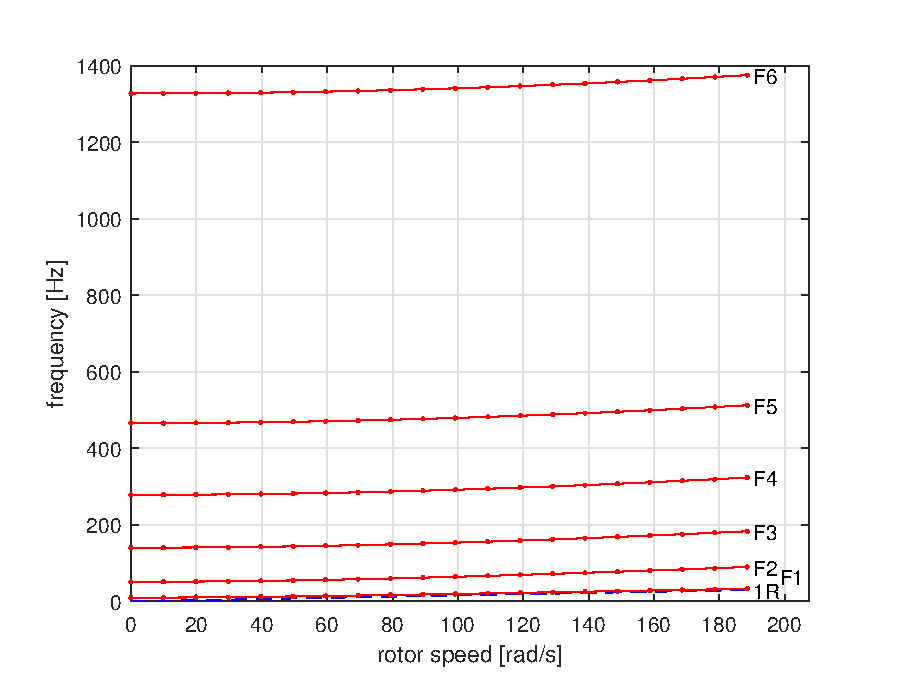
\includegraphics[width=0.43\textwidth]{FREQDIAG2.eps}}}
    \qquad
    \subfloat[\label{fig:reldiff2}Plot of the frequency margins for each harmonic, from the natural rotor frequency, with fitted curve]{{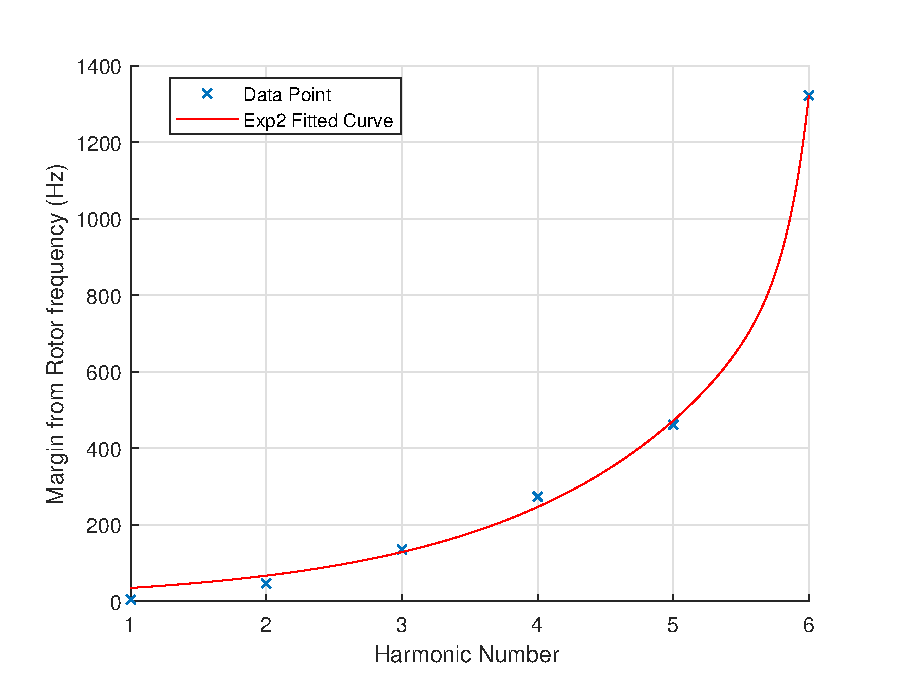
\includegraphics[width=0.43\textwidth]{RelDiff2.eps}}}
    \caption{Frequency diagram and relative difference plots of the first six harmonics of quadratic $EI(x)$ distribution.}
\end{figure}

\begin{figure}[H]
    \centering
    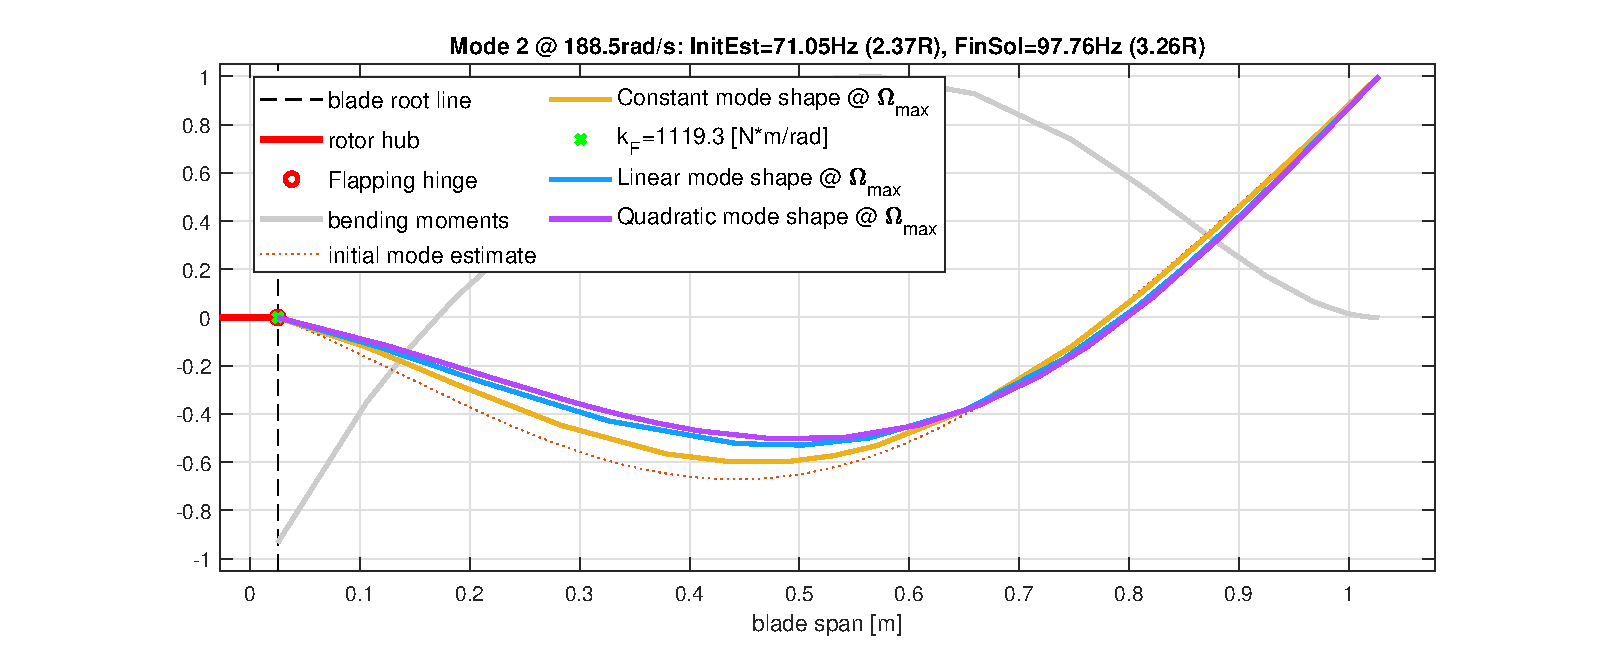
\includegraphics[width=0.85\textwidth]{mode2compare.eps}
    \caption{Comparative mode-shape plot of Constant, Linear and Quadratic $EI(x)$ distributions, second mode}
    \label{fig:bvpcomp}
\end{figure}{}
\subsection{Discussion}
%Observed trends and interesting insights, parameter effects and influences, further exploitation, …
From Figure \ref{fig:freqdiag2}, it can be seen that the general trend of the modal frequencies to increase with rotor speed has not changed, however the spacing between them and the rotor frequency is no longer represented by a quadratic curve. From Figure \ref{fig:reldiff2}, it can be seen that this relationship now more closely matches a two-term exponential function, with the sixth mode having a very high frequency in comparison to the other modes. This could be due to the reducing stiffness along the span.
From Figure \ref{fig:bvpcomp}, it can be seen that while the start and end points are the same, the frequency and amplitude of the shape differ. As the order of the distribution increases the mode shape becomes flatter and the frequency of oscillation reduces.
\section{Summary}
%Overall main findings, ways forward or possible follow up activities
In summary, the experimental phase of this exercise showed that a friction-based root condition has a higher rate of damping compared to a geometric restriction, and that loosening this increased the damping further. However this may come at the cost of large oscillations. The effect of adding tip masses was a decrease in all modal frequencies. The decrease was proportional to their absolute value. Future work may include carrying out a more controlled experiment to reduce error in the results.
The modelling phase brought to light the challenges in idealising a cantilever beam as a hinged blade. By modifying the root stiffness. data agreement between experiment and model modal frequencies was brought down to $6.68\%$, it was observed that the error increased at higher harmonics. The relative frequency margins of the modes was found to follow a quadratic curve. The BVP modelling phase highlighted the importance of understanding how solvers such as $bvp4c$ functioned. Boundary conditions for increasing orders of $EI(x)$ distribution were implemented. It was found that a higher order reduced the resulting frequency and amplitude of oscillation, although further investigation is necessary to determine the root cause of this. This may include ensuring the average value of stiffness remain the same as opposed to the concept of fixed conditions. 





%-------------------------------------------------------------------------------
% REFERENCES
%-------------------------------------------------------------------------------
\begin{thebibliography}{}
\bibitem{charts}R. Yntema, Simplified procedures and charts for the rapid estimation of bending frequencies of rotating beams. Washington, D.C.: National Advisory Committee for Aeronautics, 1955.
\bibitem{brano1}B. Titurus, Dynamics of Rotors - Experimental Blade Modal Analysis. Bristol, UK. : University of Bristol, 2019
\bibitem{bvp}J. Kierzenka and L. Shampine, "A BVP solver based on residual control and the Maltab PSE", ACM Transactions on Mathematical Software, vol. 27, no. 3, pp. 299-316, 2001. Available: 10.1145/502800.502801 [Accessed 21 November 2019].
\end{thebibliography}{}
%-------------------------------------------------------------------------------
% APPENDIX
%-------------------------------------------------------------------------------
\appendix
%\addcontentsline{toc}{section}{APPENDIX}
\renewcommand\thefigure{A.\arabic{figure}}  
\setcounter{figure}{0}



\end{document}




%-------------------------------------------------------------------------------
% SNIPPETS
%-------------------------------------------------------------------------------

% \begin{figure}[!ht]
% 	\centering
% 	\includegraphics[width=0.8\textwidth]{file_name}
% 	\caption{}
% 	\centering
% 	\label{label:file_name}
% \end{figure}

%\begin{figure}[!ht]
%	\centering
%	\includegraphics[width=0.8\textwidth]{graph}
%	\caption{Blood pressure ranges and associated level of hypertension (American Heart Association, 2013).}
%	\centering
%	\label{label:graph}
%\end{figure}

%\begin{wrapfigure}{r}{0.30\textwidth}
%	\vspace{-40pt}
%	\begin{center}
%		\includegraphics[width=0.29\textwidth]{file_name}
%	\end{center}
%	\vspace{-20pt}
%	\caption{}
%	\label{label:file_name}
%\end{wrapfigure}

%\begin{wrapfigure}{r}{0.45\textwidth}
%	\begin{center}
%		\includegraphics[width=0.29\textwidth]{manometer}
%	\end{center}
%	\caption{Aneroid sphygmomanometer with stethoscope (Medicalexpo, 2012).}
%	\label{label:manometer}
%\end{wrapfigure}

%\begin{table}[!ht]\footnotesize
%	\centering
%	\begin{tabular}{cccccc}
%	\toprule
%	\multicolumn{2}{c} {Pearson's correlation test} & \multicolumn{4}{c} {Independent t-test} \\
%	\midrule	
%	\multicolumn{2}{c} {Gender} & \multicolumn{2}{c} {Activity level} & \multicolumn{2}{c} {Gender} \\
%	\midrule
%	Males & Females & 1st level & 6th level & Males & Females \\
%	\midrule
%	\multicolumn{2}{c} {BMI vs. SP} & \multicolumn{2}{c} {Systolic pressure} & \multicolumn{2}{c} {Systolic Pressure} \\
%	\multicolumn{2}{c} {BMI vs. DP} & \multicolumn{2}{c} {Diastolic pressure} & \multicolumn{2}{c} {Diastolic pressure} \\
%	\multicolumn{2}{c} {BMI vs. MAP} & \multicolumn{2}{c} {MAP} & \multicolumn{2}{c} {MAP} \\
%	\multicolumn{2}{c} {W:H ratio vs. SP} & \multicolumn{2}{c} {BMI} & \multicolumn{2}{c} {BMI} \\
%	\multicolumn{2}{c} {W:H ratio vs. DP} & \multicolumn{2}{c} {W:H ratio} & \multicolumn{2}{c} {W:H ratio} \\
%	\multicolumn{2}{c} {W:H ratio vs. MAP} & \multicolumn{2}{c} {\% Body fat} & \multicolumn{2}{c} {\% Body fat} \\
%	\multicolumn{2}{c} {} & \multicolumn{2}{c} {Height} & \multicolumn{2}{c} {Height} \\
%	\multicolumn{2}{c} {} & \multicolumn{2}{c} {Weight} & \multicolumn{2}{c} {Weight} \\
%	\multicolumn{2}{c} {} & \multicolumn{2}{c} {Heart rate} & \multicolumn{2}{c} {Heart rate} \\
%	\bottomrule
%	\end{tabular}
%	\caption{Parameters that were analysed and related statistical test performed for current study. BMI - body mass index; SP - systolic pressure; DP - diastolic pressure; MAP - mean arterial pressure; W:H ratio - waist to hip ratio.}
%	\label{label:tests}
%\end{table}
